\documentclass[tikz,border=10pt]{standalone}

\usepackage{amsmath,amssymb,bm}
\usetikzlibrary{
    arrows.meta,
    positioning,
    shapes.geometric
}

\begin{document}

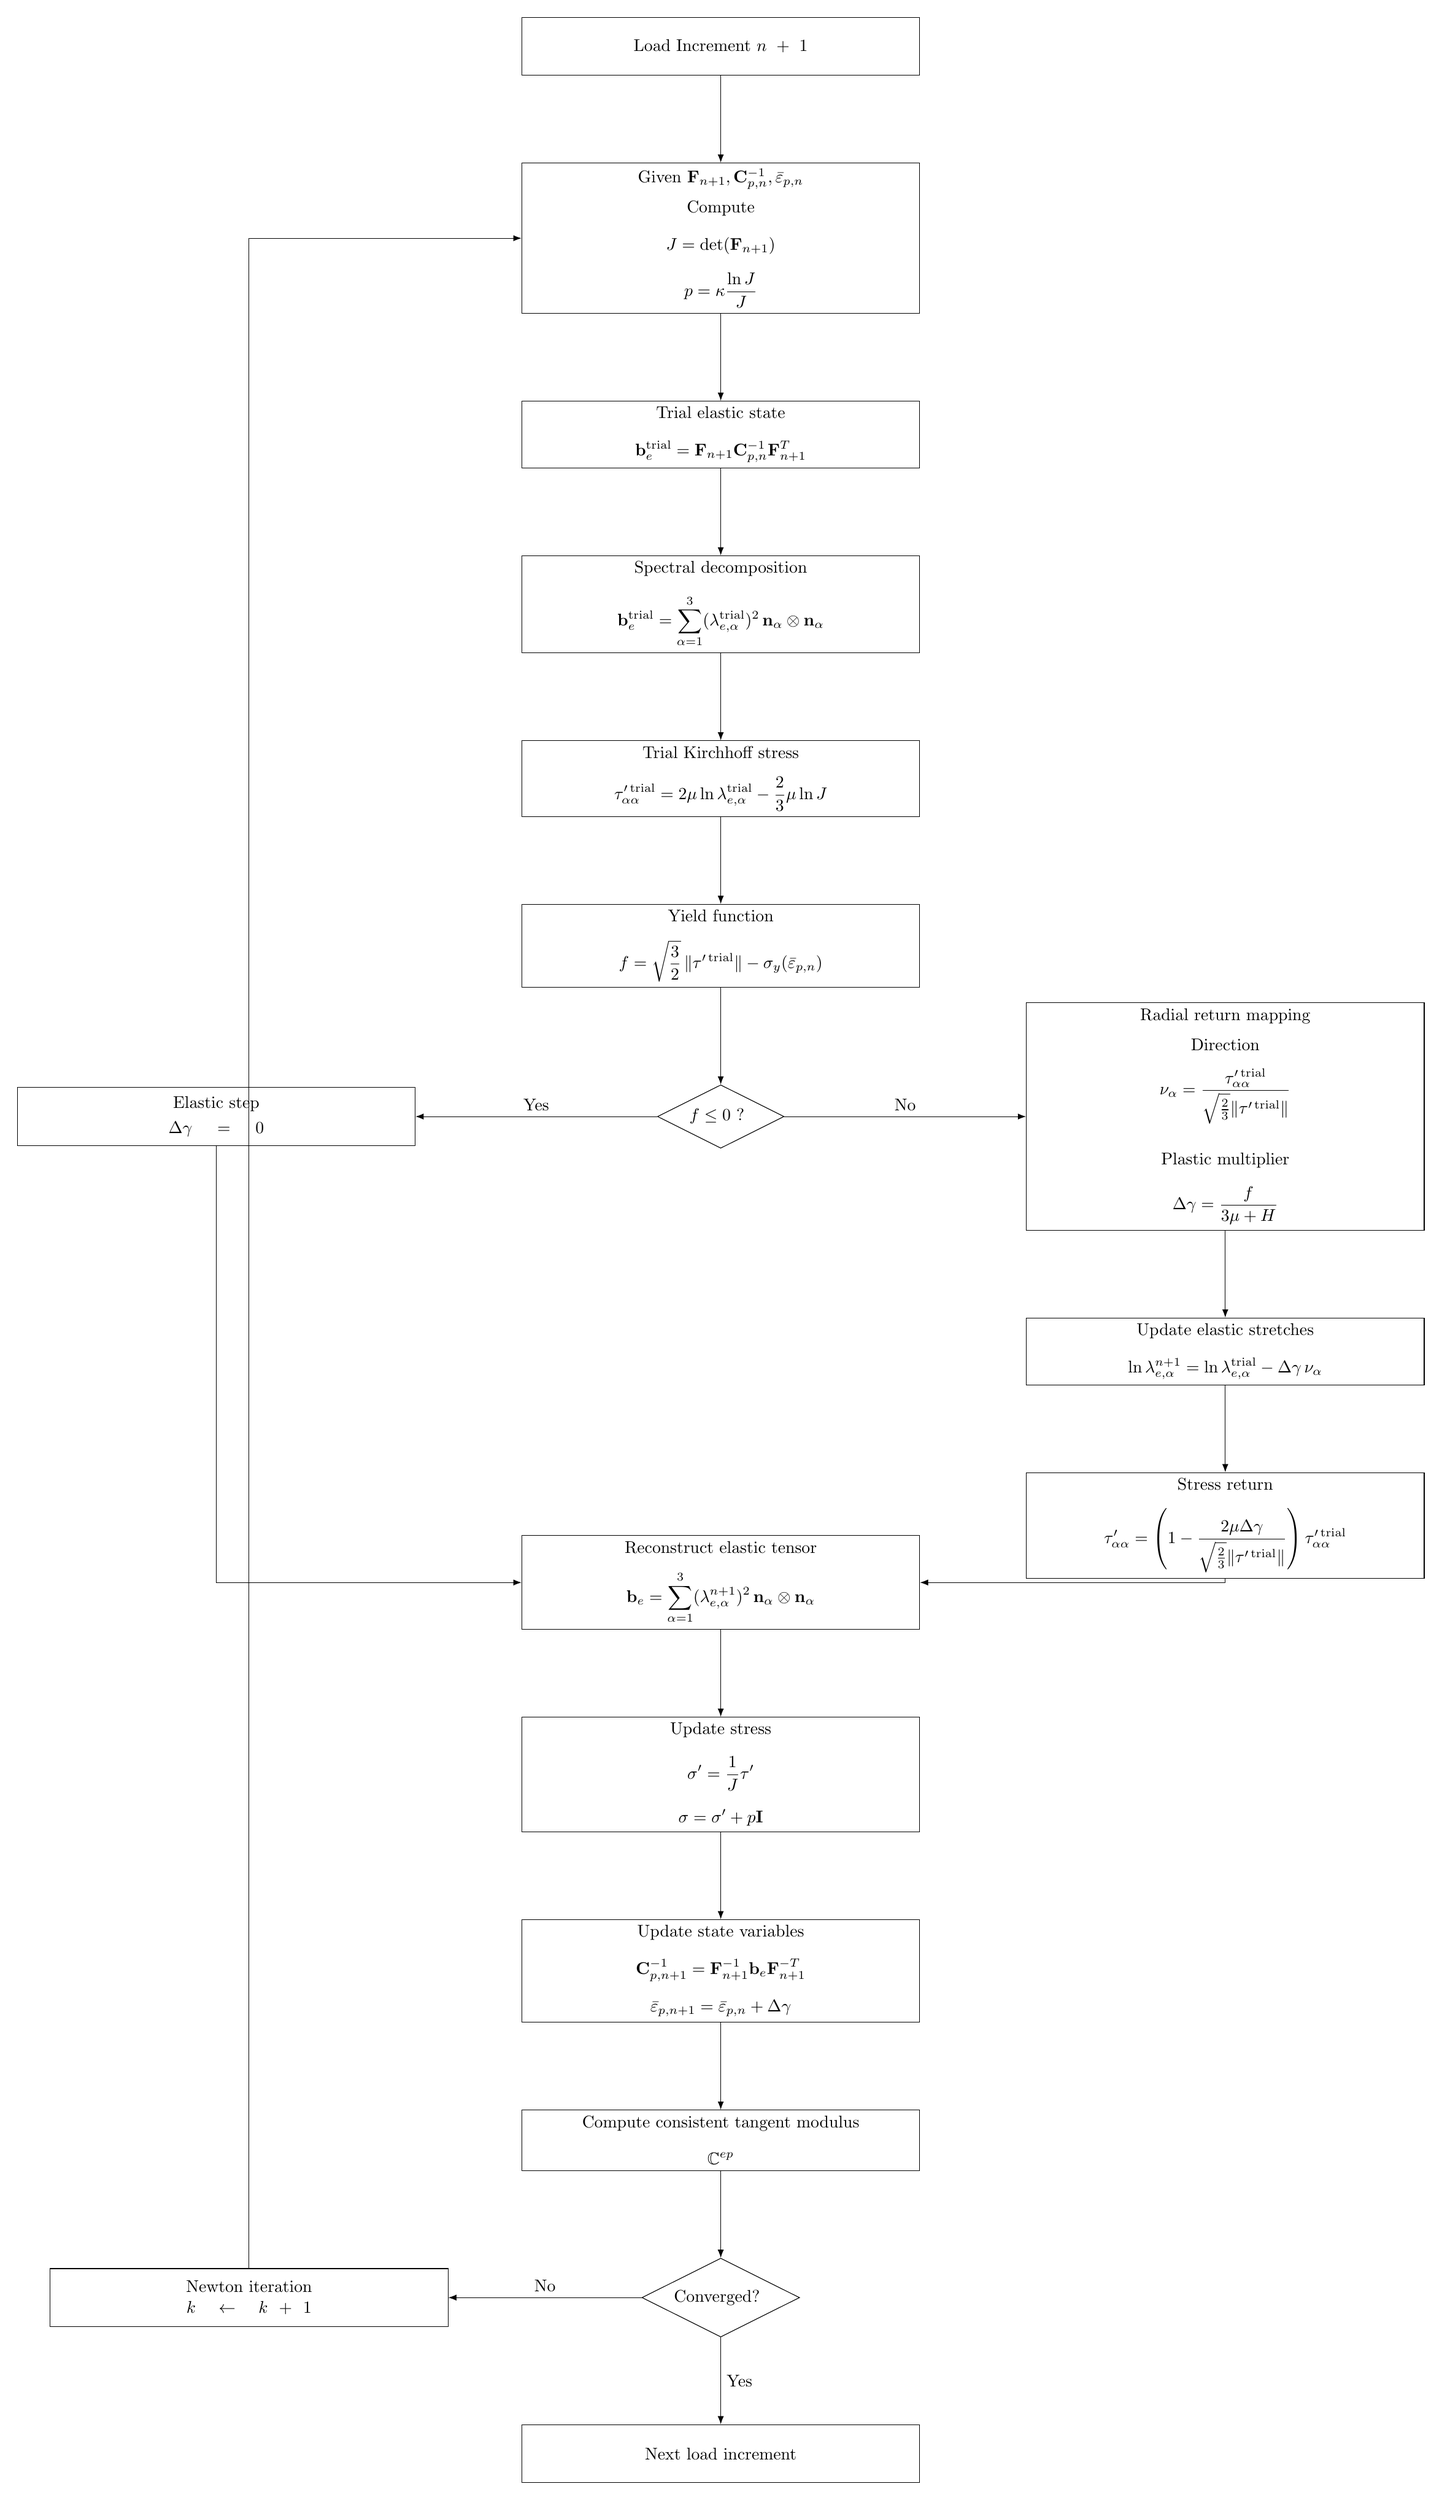
\begin{tikzpicture}[
    node distance=1.8cm,
    >=Latex,
    block/.style={
        rectangle,
        draw,
        align=center,
        text width=8cm,
        minimum height=1.2cm
    },
    decision/.style={
        diamond,
        draw,
        aspect=2,
        align=center
    }
]

%--------------------------------------------------
\node[block] (start)
{
Load Increment $n+1$
};

\node[block,below=of start] (trial)
{
Given
$
\mathbf F_{n+1},
\mathbf C^{-1}_{p,n},
\bar\varepsilon_{p,n}
$
\\[2mm]
Compute
\[
J=\det(\mathbf F_{n+1})
\]
\[
p=\kappa\frac{\ln J}{J}
\]
};

\node[block,below=of trial] (be)
{
Trial elastic state
\[
\mathbf b_e^{\mathrm{trial}}
=
\mathbf F_{n+1}
\mathbf C^{-1}_{p,n}
\mathbf F_{n+1}^{T}
\]
};

\node[block,below=of be] (spectral)
{
Spectral decomposition
\[
\mathbf b_e^{\mathrm{trial}}
=
\sum_{\alpha=1}^{3}
(\lambda^{\mathrm{trial}}_{e,\alpha})^2
\,
\mathbf n_\alpha
\otimes
\mathbf n_\alpha
\]
};

\node[block,below=of spectral] (stress)
{
Trial Kirchhoff stress
\[
\tau_{\alpha\alpha}^{\prime\,\mathrm{trial}}
=
2\mu
\ln\lambda^{\mathrm{trial}}_{e,\alpha}
-
\frac23\mu\ln J
\]
};

\node[block,below=of stress] (yield)
{
Yield function
\[
f
=
\sqrt{\frac32}
\,
\|\tau^{\prime\,\mathrm{trial}}\|
-
\sigma_y(\bar\varepsilon_{p,n})
\]
};

\node[decision,below=2cm of yield] (check)
{
$f\le 0$ ?
};

% Elastic
\node[block,left=5cm of check] (elastic)
{
Elastic step
\\[1mm]
$\Delta\gamma=0$
};

% Plastic
\node[block,right=5cm of check] (plastic)
{
Radial return mapping
\\[2mm]
Direction
\[
\nu_\alpha
=
\frac{
\tau^{\prime\,\mathrm{trial}}_{\alpha\alpha}
}{
\sqrt{\frac23}
\|\tau^{\prime\,\mathrm{trial}}\|
}
\]
\\[2mm]
Plastic multiplier
\[
\Delta\gamma
=
\frac{
f
}{
3\mu+H
}
\]
};

\node[block,below=of plastic] (update_lambda)
{
Update elastic stretches
\[
\ln\lambda_{e,\alpha}^{n+1}
=
\ln\lambda_{e,\alpha}^{\mathrm{trial}}
-
\Delta\gamma\,\nu_\alpha
\]
};

\node[block,below=of update_lambda] (update_tau)
{
Stress return
\[
\tau'_{\alpha\alpha}
=
\left(
1-
\frac{
2\mu\Delta\gamma
}{
\sqrt{\frac23}
\|\tau^{\prime\,\mathrm{trial}}\|
}
\right)
\tau^{\prime\,\mathrm{trial}}_{\alpha\alpha}
\]
};

\node[block,below=8cm of check] (be_update)
{
Reconstruct elastic tensor
\[
\mathbf b_e
=
\sum_{\alpha=1}^{3}
(\lambda^{n+1}_{e,\alpha})^2
\,
\mathbf n_\alpha
\otimes
\mathbf n_\alpha
\]
};

\node[block,below=of be_update] (sigma)
{
Update stress
\[
\sigma'
=
\frac1J\tau'
\]
\[
\sigma
=
\sigma'
+
p\mathbf I
\]
};

\node[block,below=of sigma] (state)
{
Update state variables
\[
\mathbf C^{-1}_{p,n+1}
=
\mathbf F^{-1}_{n+1}
\mathbf b_e
\mathbf F^{-T}_{n+1}
\]
\[
\bar\varepsilon_{p,n+1}
=
\bar\varepsilon_{p,n}
+
\Delta\gamma
\]
};

\node[block,below=of state] (tangent)
{
Compute consistent tangent modulus
\[
\mathbb C^{ep}
\]
};

\node[decision,below=of tangent] (conv)
{
Converged?
};

\node[block,left=4cm of conv] (iter)
{
Newton iteration
\\
$k\leftarrow k+1$
};

\node[block,below=of conv] (end)
{
Next load increment
};

%--------------------------------------------------
\draw[->] (start) -- (trial);
\draw[->] (trial) -- (be);
\draw[->] (be) -- (spectral);
\draw[->] (spectral) -- (stress);
\draw[->] (stress) -- (yield);
\draw[->] (yield) -- (check);

\draw[->] (check) -- node[above]{Yes} (elastic);
\draw[->] (check) -- node[above]{No} (plastic);

\draw[->] (plastic) -- (update_lambda);
\draw[->] (update_lambda) -- (update_tau);

\draw[->] (elastic) |- (be_update);
\draw[->] (update_tau) |- (be_update);

\draw[->] (be_update) -- (sigma);
\draw[->] (sigma) -- (state);
\draw[->] (state) -- (tangent);
\draw[->] (tangent) -- (conv);

\draw[->] (conv) -- node[above]{No} (iter);
\draw[->] (iter) |- (trial);

\draw[->] (conv) -- node[right]{Yes} (end);

\end{tikzpicture}

\end{document}

